\documentclass[a4paper]{article}

\RequirePackage{graphicx}
\usepackage{authblk}
\usepackage{cleveref}
\crefname{figure}{figure}{figures}
\usepackage{caption}
\usepackage[dvipsnames]{xcolor}
%\usepackage{subcaption}
\usepackage[UKenglish]{babel}
\usepackage{alltt}
\usepackage{afterpage}
\usepackage[text={16cm,25cm},centering]{geometry}
\usepackage{enumitem}
\setenumerate[1]{label=Req. \thesubsection.\arabic*.}
\setenumerate[2]{label=\arabic*.}

%\geometry{
%  a4paper,%
%  top=3cm,%
%  textwidth=16cm,% 
%  textheight=23.2cm,%
%  marginparsep=7pt,% 
%  marginparwidth=2.5cm%
%}

\renewcommand*{\familydefault}{\sfdefault}

\title{Specification for the SoLid read-out electronics}
\author[]{SoLid read-out team}
\date{\today\\V0.1}

\newcommand{\must}[1]{\textcolor{red}{#1}}
\newcommand{\should}[1]{\textcolor{orange}{#1}}
\def\I2C{I$^2$C}


\begin{document}


\maketitle

\tableofcontents

\section{Introduction}

\begin{itemize}
    \item Overview of system
    \item Description of which parts of system are covered by this spec
    \item Lay out of spec
\end{itemize}

\section{PCB specifications}

The specifications for the various PCBs that will be designed are given in the following subsections.

\clearpage
\newpage
\subsection{SiPM board}

{\bf Designer: Nick Ryder}

The SiPM boards each house a single SiPM and a connect to two twisted pairs of the SiPM ribbon cable.
One pair provides the bias voltage for the SiPM, the other acts as a ground/voltage reference.

\begin{figure}[h]
    \begin{center}
        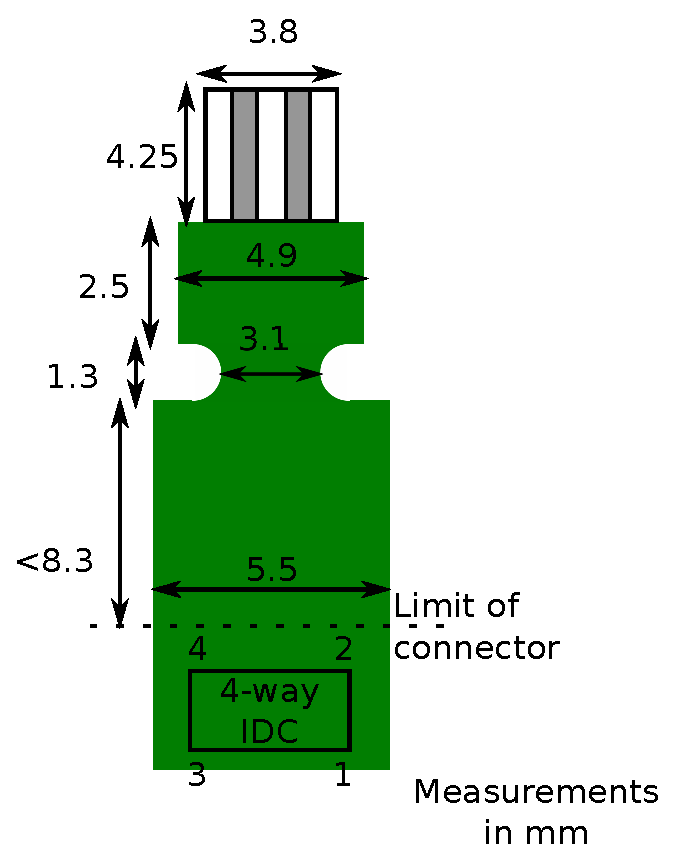
\includegraphics[width=0.4\textwidth]{imgs/sipmboardsize}
        \caption{Size of the SiPM board.}
        \label{fig:sipmboardsize}
    \end{center}
\end{figure}


\begin{table}[h]
    \begin{center}
        \caption{Pin mapping for the 4-way IDC socket on the SiPM board.}
        \label{tab:IDC4waySiPM}
        \begin{tabular}{cc}
            \hline
            \hline
            Pin & Function \\
            \hline
            1 & HV? \\
            2 & LV? \\
            3 & GND? \\
            4 & GND? \\
            \hline
            \hline
        \end{tabular}
    \end{center}
\end{table}

\begin{enumerate}
    \item \must{The SiPM board must fit within the existing 3D printed socket design, with dimensions as shown in \cref{fig:sipmboardsize}.}
    \item \must{The SiPM board must house a single S12752-050P SiPM.}
    \item \must{The SiPM board must connect to the SiPM ribbon cable using a 4-way 1.27 mm pitch IDC socket (Farnell XXXXXX).}
    \item \must{The socket pin connections must be as detailed in \cref{tab:IDC4waySiPM}.}
    \item \should{The SiPM boards should be designed to ease the production of 3000 units.}
    \item \should{The PCB silkscreen should indicate which order the ribbon cable wires (either coloured or brown) correspond to the IDC socket.}
\end{enumerate}

\clearpage
\newpage
\subsection{In-detector sensors}

{\bf Designer: ???}

An \I2C bus will be provided on a twisted pair ribbon cable within the detector to allow deployment of sensors within the detector frame.
Temperature sensors will be deployed within the frame.
Other sensors or systems such as humidity sensors or LED flashers may also be deployed.

\begin{table}[h]
    \begin{center}
        \caption{Pin mapping for the 4-way IDC socket on the sensor board.}
        \label{tab:IDC4waySensor}
        \begin{tabular}{cc}
            \hline
            \hline
            Pin & Function \\
            \hline
            1 & 3.3 V? \\
            2 & GND? \\
            3 & SCL? \\
            4 & SDA? \\
            \hline
            \hline
        \end{tabular}
    \end{center}
\end{table}

\begin{enumerate}
    \item \must{The sensor board must connect to the SiPM ribbon cable using a 4-way 1.27 mm pitch IDC socket (Farnell XXXXXXX).}
    \item \must{The socket pin connections must be as detailed in \cref{tab:IDC4waySensor}.}
    \item \must{Each sensor board should allow the selection of \I2C addresses per sensor.}
    \item \should{Sensor addresses should not clash with the temperature sensors on the analog board.}
\end{enumerate}

\clearpage
\newpage
\subsection{Analog board}

{\bf Designer: Wim Beaumont}

The analog boards provide a programmable bias voltage to each SiPM and also amplify the signals from each SiPM.
Two analog boards will be used per detector plane.
All analog boards are identical.

\begin{figure}[h]
    \begin{center}
        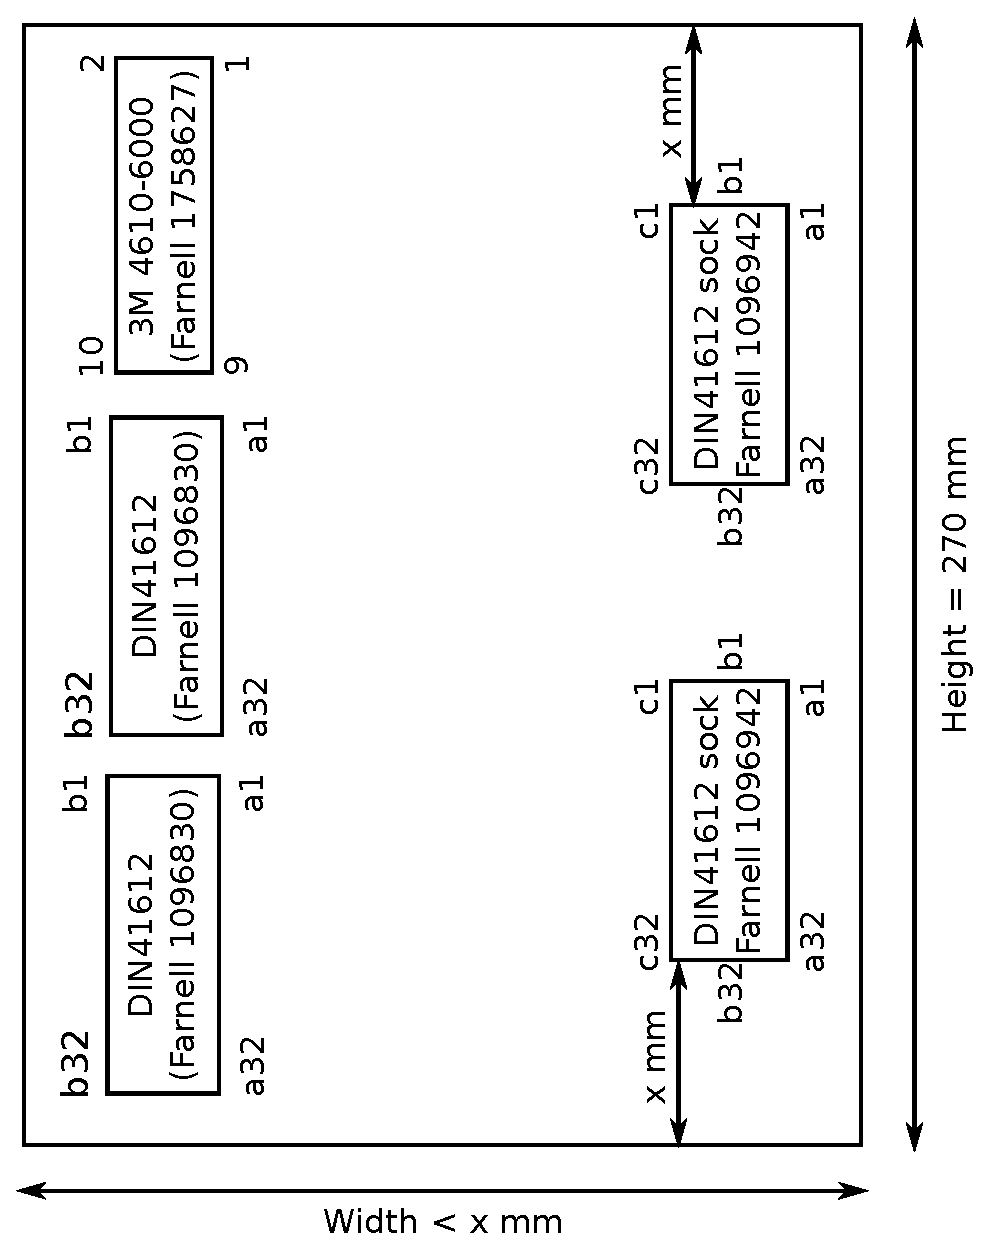
\includegraphics[width=0.8\textwidth]{imgs/analogboardsize}
        \caption{Size of the analog board and positions of connectors.}
        \label{fig:analogboardsize}
    \end{center}
\end{figure}

\begin{figure}[h]
    \begin{center}
        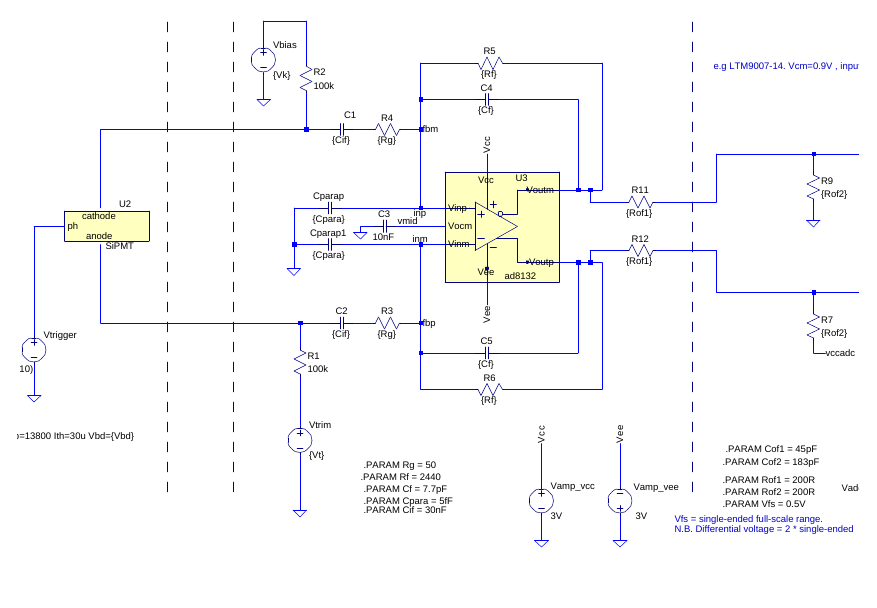
\includegraphics[width=0.8\textwidth]{imgs/SiPM_test_dc_schematic}
        \caption{Amplifier circuit design.}
        \label{fig:amplifiercircuit}
    \end{center}
\end{figure}

\begin{table}[h]
    \begin{center}
        \caption{Pin mapping for the 64-way DIN41612 socket housed on the analog board for connecting to the SiPM ribbon cable. The pin pattern is repeated 16 times.}
        \label{tab:IDC64way}
        \begin{tabular}{cc}
            \hline
            \hline
            Pin & Function \\
            \hline
            1 + 4N & SiPM HV? \\
            2 + 4N & SiPM LV? \\
            3 + 4N & GND? \\
            4 + 4N & GND? \\
            \hline
            \hline
        \end{tabular}
    \end{center}
\end{table}

\begin{table}[h]
    \begin{center}
        \caption{Pin mapping for the 10-way IDC socket housed on the analog board for connecting to the in-detector I2C bus.}
        \label{tab:IDC10way}
        \begin{tabular}{cc|cc|cc|cc|cc}
            \hline
            \hline
            Pin & Function & Pin & Function & Pin & Function & Pin & Function & Pin & Function \\
            \hline
            1 & 3.3 V? & 3 & SCL? & 5 & NC & 7 & 3.3 V? & 9 & SCL? \\
            2 & GND? & 4 & SDA? & 6 & NC & 8 & GND? & 10 & SDA? \\
            \hline
            \hline
        \end{tabular}
    \end{center}
\end{table}

\begin{table}[h]
    \begin{center}
        \caption{Pin mapping for the upper 96-way DIN socket connecting the analog to the digital board.}
        \label{tab:DIN96Upper}
        \begin{tabular}{cc|cc|cc}
            \hline
            \hline
            Pin & Function & Pin & Function & Pin & Function \\
            \hline
            A1 & x & B1 & y & C1 & z \\
            A2 & x & B2 & y & C2 & z \\
            A3 & x & B3 & y & C3 & z \\
            A4 & x & B4 & y & C4 & z \\
            A5 & x & B5 & y & C5 & z \\
            A6 & x & B6 & y & C6 & z \\
            A7 & x & B7 & y & C7 & z \\
            A8 & x & B8 & y & C8 & z \\
            A9 & x & B9 & y & C9 & z \\
            A10 & x & B10 & y & C10 & z \\
            A11 & x & B11 & y & C11 & z \\
            A12 & x & B12 & y & C12 & z \\
            A13 & x & B13 & y & C13 & z \\
            A14 & x & B14 & y & C14 & z \\
            A15 & x & B15 & y & C15 & z \\
            A16 & x & B16 & y & C16 & z \\
            A17 & x & B17 & y & C17 & z \\
            A18 & x & B18 & y & C18 & z \\
            A19 & x & B19 & y & C19 & z \\
            A20 & x & B20 & y & C20 & z \\
            A21 & x & B21 & y & C21 & z \\
            A22 & x & B22 & y & C22 & z \\
            A23 & x & B23 & y & C23 & z \\
            A24 & x & B24 & y & C24 & z \\
            A25 & x & B25 & y & C25 & z \\
            A26 & x & B26 & y & C26 & z \\
            A27 & x & B27 & y & C27 & z \\
            A28 & x & B28 & y & C28 & z \\
            A29 & x & B29 & y & C29 & z \\
            A30 & x & B30 & y & C30 & z \\
            A31 & x & B31 & y & C31 & z \\
            A32 & x & B32 & y & C32 & z \\
            \hline
            \hline
        \end{tabular}
    \end{center}
\end{table}

\begin{table}[h]
    \begin{center}
        \caption{Pin mapping for the upper 96-way DIN socket connecting the analog to the digital board.}
        \label{tab:DIN96Lower}
        \begin{tabular}{cc|cc|cc}
            \hline
            \hline
            Pin & Function & Pin & Function & Pin & Function \\
            \hline
            A1 & x & B1 & y & C1 & z \\
            A2 & x & B2 & y & C2 & z \\
            A3 & x & B3 & y & C3 & z \\
            A4 & x & B4 & y & C4 & z \\
            A5 & x & B5 & y & C5 & z \\
            A6 & x & B6 & y & C6 & z \\
            A7 & x & B7 & y & C7 & z \\
            A8 & x & B8 & y & C8 & z \\
            A9 & x & B9 & y & C9 & z \\
            A10 & x & B10 & y & C10 & z \\
            A11 & x & B11 & y & C11 & z \\
            A12 & x & B12 & y & C12 & z \\
            A13 & x & B13 & y & C13 & z \\
            A14 & x & B14 & y & C14 & z \\
            A15 & x & B15 & y & C15 & z \\
            A16 & x & B16 & y & C16 & z \\
            A17 & x & B17 & y & C17 & z \\
            A18 & x & B18 & y & C18 & z \\
            A19 & x & B19 & y & C19 & z \\
            A20 & x & B20 & y & C20 & z \\
            A21 & x & B21 & y & C21 & z \\
            A22 & x & B22 & y & C22 & z \\
            A23 & x & B23 & y & C23 & z \\
            A24 & x & B24 & y & C24 & z \\
            A25 & x & B25 & y & C25 & z \\
            A26 & x & B26 & y & C26 & z \\
            A27 & x & B27 & y & C27 & z \\
            A28 & x & B28 & y & C28 & z \\
            A29 & x & B29 & y & C29 & z \\
            A30 & x & B30 & y & C30 & z \\
            A31 & x & B31 & y & C31 & z \\
            A32 & x & B32 & y & C32 & z \\
            \hline
            \hline
        \end{tabular}
    \end{center}
\end{table}

\begin{enumerate}
    \item \must{The analog board height (as shown in \cref{fig:analogboardsize}) must be 270 mm.}
    \item \should{The analog board width should be less than xx mm.}
    \item \must{The analog board must connect two two 16-SiPM ribbon cables via a 64-way 1.27mm pitch DIN41612 plug connector each (Farnell 1096830).}
    \item \must{The pin mapping for each IDC socket connectiong to the SiPM ribbon cables must be as described in \cref{tab:IDC64way}.}
    \item \must{The analog board must connect to two in-detector I2C buses via a 10-way IDC socket (Farnell 1758627).}
    \item \must{The pin mapping for the connector to the in-detector I2C bus must be as shown in \cref{tab:IDC10way}.}
    \item \must{The analog board must connect to the digital board using two 96-way DIN41612 socket connectors (Farnell 1096942).}
    \item \must{The pin mapping for the two connectors to the digital board must be as described in \cref{tab:DIN96Upper,tab:DIN96Lower}.}
    \item \must{The position of the two connectors to the digital board must be as shown in \cref{fig:analogboardsize}.}
    \item \must{The analog board must use input power connections of -5, GND, + 7 V.}
    \item \must{The analog board must regulate the input power to -3, GND, +5 V using linear regulators.}
    \item \must{The regulators must be controllable from the digital board to enable or disable powering the analog board components.}
    \item \must{The analog board must amplifier the signal from each of 32 SiPMs using an AD8132 amplifier, using the circuit as shown in \cref{fig:amplifiercircuit}.}
    \item \must{The analog board must be compatible with replacing the DC connection to the digital board with an AC connection by replacing only passive components and not using the negative voltage power supply.}
    \item \must{The analog board must be able to produce a programmable high voltage bias supply on board, using ADL5317.}
    \item \must{The analog board must provide a per SiPM low voltage trim using programmable DACs.}
    \item \must{The ananlog board must provide an on-board temperature measurement and unique ID using a XXX chip with an \I2C address of 0bXXXXXXX.} 
\end{enumerate}

\clearpage
\newpage

\subsection{Digital board}

{\bf Designer: David Cussans}

The digital boards house an FPGA board which does front end processing and triggering.
They also digitise the amplified signals from the analog boards.
There are two variants of the digital board, one of each will be deployed in each module.
The `master' board will receive all Ethernet traffic for the two boards, with traffic passed to the `slave' via a serial link.
The slave board will not have an Ethernet link, but will be upgradable to have one if needed.
The master will also receive the clock and synchronisation signals for the module and fan them out to the slave board.

{\bf Add a diagram of master/slave}

\begin{figure}[h]
    \begin{center}
        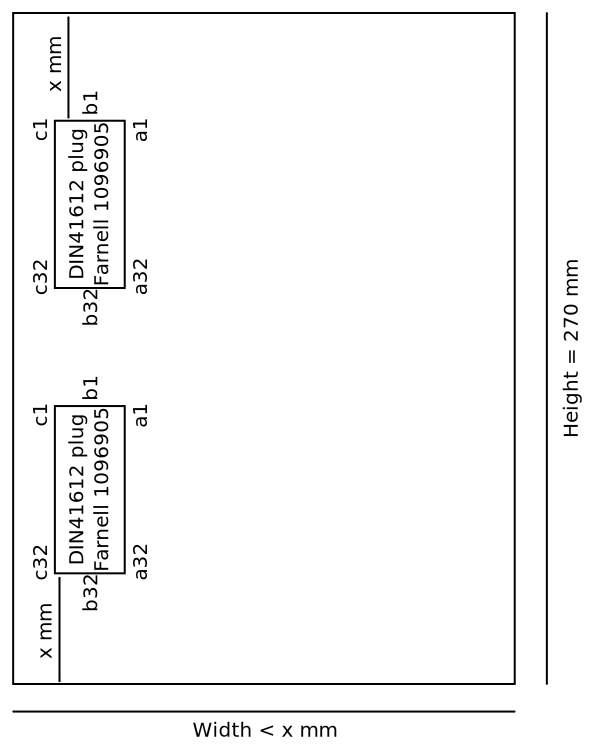
\includegraphics[width=0.8\textwidth]{imgs/digitalboardsize}
        \caption{Size of the digital board and positions of connectors.}
        \label{fig:digitalboardsize}
    \end{center}
\end{figure}

\begin{table}[h]
    \begin{center}
        \caption{Pin information for the Trenz FPGA board.}
        \label{tab:TrenzPins}
        \begin{tabular}{cc}
            \hline
            \hline
            Pins & Functions \\
            \hline
            A & x \\
            B & y \\
            \hline
            \hline
        \end{tabular}
    \end{center}
\end{table}

\begin{table}[h]
    \begin{center}
        \caption{Pin information for the eSATA connector used for the clock and synchronisation signals.}
        \label{tab:ClockSyncPins}
        \begin{tabular}{cc}
            \hline
            \hline
            Pins & Functions \\
            \hline
            1 & GND? \\
            2 & CLK+? \\
            3 & CLK-? \\
            4 & GND? \\
            5 & Sync+? \\
            6 & Sync-? \\
            7 & GND? \\
            \hline
            \hline
        \end{tabular}
    \end{center}
\end{table}


\begin{enumerate}
    \item \must{The digital board height (as shown in \cref{fig:digitalboardsize}) must be 270 mm.}
    \item \should{The digital board width should be less than xx mm.}
    \item \must{The digital board must connect to the digital board using two 96-way DIN41612 plug connectors (Farnell 1096905).}
    \item \must{The pin mapping for the connectors to the analog board must be as described in \cref{tab:DIN96Upper,tab:DIN96Lower}.}
    \item \must{The position of the two 96-way DIN41612 connectors must be as shown in \cref{fig:digitalboardsize}.}
    \item \must{The digital board must allow a Trenz XXX board to be plugged in using two XXXX connectors.}
    \item \must{The pin mapping for the Trenz board connections must be as shown in \cref{tab:TrenzPins}.}
    \item \must{The digital board must digitise 32 SiPM channels using multiple XXXX ADCs.}
    \item \must{The ADCs must be controlled via N SPI buses, with two chip select lines per ADC chip.}
    \item \must{The master digital board must have an HDMI connector to receive a clock and synchronisation signal.}
    \item \must{The master digital board must fan out the clock and synchronisation signals to the slave digital board.}
    \item \must{The digital board must have an on board Si5326 chip to clean the external clock signal and provide the clocks for the ADC chips and FPGA.}
    \item \must{The Si5326 clock chip must be controlled by an \I2C bus on the digital board.}
    \item \must{The digital board must have an SFP+ cage for a Gbps Ethernet connection.}
    \item \must{The digital board must use input power connections of GND and 48 V.}
    \item \must{The digital board must convert the input power to 1.8 V, 3.3 V, x V using on-board switching DC-DC converters.}
    \item \must{The DC-DC converters must be controllable from the FPGA, to enable/disable powering of the ADC.}
    \item \must{The digital board should include a temperature sensor that can power down the FPGA if the board temperature exceeds a programmable alarm threshold.}
    \item \must{The digital board must have two eSATA sockets to allow Gbps serial communications between FPGAs.}
\end{enumerate}

\clearpage
\newpage
\subsection{Clock distribution board}

{\bf Designer: David Cussans}

The clock distribution board provides the same clock to all digital boards.
In addition the board is able to provide a synchronous pulsed signal to all boards to ensure synchronisation across the detector.

\begin{enumerate}
    \item \must{The clock distribution board must provide a xxx MHz clock to all digital boards.}
    \item \must{The clock distribution board must provide a programmable pulse signal synchronously to all digital boards.}
    \item \must{The clock and synchronisation signals must be provided via an eSATA connector.}
    \item \must{The HDMI connector pin mapping must be as shown in \cref{tab:ClockSyncPins}.}
    \item \should{The FPGA controlling the clock system should have a firmware tool chain compatible with the Artix-7 that will be used on the read-out board.}
\end{enumerate}

\clearpage
\newpage

\section{Review process}

\begin{itemize}
    \item Internal review of schematics before layout:
    \begin{itemize}
        \item Check connector pin compatibility, etc.
        \item Different times for different boards.
        \item Responsible person to sign off: Alfons?
    \end{itemize}
    \item Internal + external review once design done before ordering initial boards:
    \begin{itemize}
        \item Review to include these boards and wider system design
        \item External reviewers with similar experience from RAL, Imperial, other?
    \end{itemize}
\end{itemize}

\section{Time schedule}

\begin{itemize}
    \item Design work
    \item Review system design by {\bf DATE}
    \item Produce O(10) test boards
    \item Test at least full plane at Gent
    \item Produce O(100) boards
    \item Deploy at Gent
    \item Relocate detector to BR2
\end{itemize}

\end{document}
